\documentclass[a4paper,12pt]{article}
\usepackage{amsmath}
\usepackage{amssymb,amsthm,graphicx}
\usepackage{titlesec}
\usepackage{textcomp}
\usepackage{enumitem}
\usepackage{color}
\usepackage{epsfig}
\usepackage{graphics}
\usepackage{pdfpages}
\usepackage{subcaption}
\usepackage[font=small]{caption}
\usepackage[hang,flushmargin]{footmisc} 
\usepackage{float}
\usepackage{rotating,tabularx}
\usepackage{booktabs}
\usepackage[mathscr]{euscript}
\usepackage{natbib}
\usepackage{setspace}
\usepackage{mathrsfs}
\usepackage[official]{eurosym}
\usepackage[left=2.8cm,right=2.8cm,bottom=2.8cm,top=2.5cm]{geometry}

\setcounter{secnumdepth}{4}
\renewcommand{\baselinestretch}{1.2}
\parindent0pt


% General

\newcommand{\reals}{\mathbb{R}}
\newcommand{\integers}{\mathbb{Z}}
\newcommand{\naturals}{\mathbb{N}}

\newcommand{\pr}{\mathbb{P}}        % probability
\newcommand{\ex}{\mathbb{E}}        % expectation
\newcommand{\var}{\textnormal{Var}} % variance
\newcommand{\cov}{\textnormal{Cov}} % covariance

\newcommand{\law}{\mathcal{L}} % law of X
\newcommand{\normal}{N}        % normal distribution 

\newcommand{\argmax}{\textnormal{argmax}}
\newcommand{\argmin}{\textnormal{argmin}}

\newcommand{\ind}{\mathbbm{1}} % indicator function
\newcommand{\kernel}{K} % kernel function
\newcommand{\wght}{W} % kernel weight
\newcommand{\thres}{\pi} % threshold parameter


% Convergence

\newcommand{\convd}{\stackrel{d}{\longrightarrow}}              % convergence in distribution
\newcommand{\convp}{\stackrel{P}{\longrightarrow}}              % convergence in probability
\newcommand{\convas}{\stackrel{\textrm{a.s.}}{\longrightarrow}} % convergence almost surely
\newcommand{\convw}{\rightsquigarrow}                           % weak convergence


% Theorem-like declarations

\theoremstyle{plain}

\newtheorem{theorem}{Theorem}[section]
\newtheorem{prop}[theorem]{Proposition}
\newtheorem{lemma}[theorem]{Lemma}
\newtheorem{corollary}[theorem]{Corollary}
\newtheorem*{theo}{Theorem}
\newtheorem{propA}{Proposition}[section]
\newtheorem{lemmaA}[propA]{Lemma}
\newtheorem{definition}{Definition}[section]
\newtheorem{remark}{Remark}[section]
\renewcommand{\thelemmaA}{A.\arabic{lemmaA}}
\renewcommand{\thepropA}{A.\arabic{propA}}
\newtheorem*{algo}{Clustering Algorithm}


% Theorem numbering to the left

\makeatletter
\newcommand{\lefteqno}{\let\veqno\@@leqno}
\makeatother


% Heading

\newcommand{\heading}[2]
{  \setcounter{page}{1}
   \begin{center}

   \phantom{Distance to upper boundary}
   \vspace{0.5cm}

   {\LARGE \textbf{#1}}
   \vspace{0.4cm}
 
   {\LARGE \textbf{#2}}
   \end{center}
}


% Authors

\newcommand{\authors}[4]
{  \parindent0pt
   \begin{center}
      \begin{minipage}[c][2cm][c]{5cm}
      \begin{center} 
      {\large #1} 
      \vspace{0.05cm}
      
      #2 
      \end{center}
      \end{minipage}
      \begin{minipage}[c][2cm][c]{5cm}
      \begin{center} 
      {\large #3}
      \vspace{0.05cm}

      #4 
      \end{center}
      \end{minipage}
   \end{center}
}

%\newcommand{\authors}[2]
%{  \parindent0pt
%   \begin{center}
%   {\large #1} 
%   \vspace{0.1cm}
%      
%   #2 
%   \end{center}  
%}


% Version

\newcommand{\version}[1]
{  \begin{center}
   {\large #1}
   \end{center}
   \vspace{3pt}
} 










\begin{document}



\begin{center} 
{\large \bf Revision of the paper} \\[0.1cm]
{\large \bf ``Multiscale inference and long-run variance estimation} \\[0.1cm]
{\large \bf in nonparametric regression with time series errors''} 
\end{center}
\vspace{7pt}



First of all, we would like to thank the editor, the associate editor and the reviewers for their many comments and suggestions which were very helpful in improving the paper. In the revision, we have addressed all comments and have rewritten the paper accordingly. Please find our point-by-point responses below. 
%Since the revised paper includes additional material as requested by the referees (e.g. ??), it is a bit longer than the original submission. However, we are of course happy and willing to reduce the length of the paper by shifting parts of it into the online supplement if this is needed. 
Before we reply to the specific comments of the referees, we summarize the major changes in the revision.
\vspace{10pt}


\textbf{Generalization of the theoretical results.} We have extended the theoretical results as suggested by Referee 1:
\begin{enumerate}[label=(\roman*), leftmargin=0.8cm]

\item We provide a generalization of Proposition 3.3 which shows that $\mathbb{P}({E}_T^{\ell}) = (1 - \alpha_T) + o(1)$ for any sequence $\{\alpha_T\}$ of significance levels $\alpha_T \in (0,1)$. In particular, for $\alpha_T \rightarrow 0$, we get the consistency result that $\mathbb{P}({E}_T^{\ell}) \rightarrow 1$. 

\item We have generalized our estimator of the long-run error variance. The estimation procedure is shown to be valid not only for AR($p$) processes of known order $p$ but for any stationary error process $\{\varepsilon_t\}$ with an AR($\infty$) representation. This greatly extends the applicability of the estimator. 
\end{enumerate}
\vspace{3pt}


\textbf{Comparison to SiZer.} As requested by the Associate Editor, we give a clear account of the main contributions and innovations of our paper relative to the SiZer approach in the revision. Please see the new Section ?? for the details. In what follows, we summarize the main points of the new Section ??. 

Informally speaking, both our approach and SiZer (for time series) are methods to test for local increases/decreases of a nonparametric trend function $m$. The formal problem is to test the hypothesis
\[ H_0(u,h): \text{The trend } m \text{ is constant on the time interval } [u-h,u+h] \]
simultaneously for a large number of different time intervals $[u-h,u+h]$, in particular, for all intervals with $u \in I$ and $h \in H$, where $I$ is the set of locations and $H$ the set of bandwidths or scales $H$ under consideration. 

There are two versions of SiZer, a global and a row-wise one. We here discuss the global version as it is closer in spirit to our approach. We comment on the row-wise version later on. The test statistic of the global SiZer approach has the form $S_T = \max_{h \in H} S_T(h)$, where $S_T(h) = \max_{u \in I} |s_T(u,h)|$ for each scale $h$ and $s_T(u,h)$ is a test statistic for $H_0(u,h)$. As shown in Chaudhuri \& Marron (2000) for the i.i.d.\ case and in Park et al.\ (2009) for the dependent data case, $S_T$ weakly converges to some limit process $S$ under the overall null hypothesis $H_0$ that $H_0(u,h)$ is fulfilled for all $u \in I$ and $h \in H$. Using this result, one can take the $(1-\alpha)$-quantile of $S$ as a critical value of the SiZer test. (As this quantile can usually not be determined analytically, it has to be approximated, e.g., by the bootstrap procedures of Chaudhuri \& Marron (2000) or the extreme value theory based procedure of Hannig \& Marron (2006).)

Even though related, our methods and theory are very different from those in the SiZer literature:
\begin{itemize}[leftmargin=0.5cm]

\item Theory for SiZer is derived under the assumption that $H$ is a compact subset of $(0,1)$. As already pointed out in Chaudhuri \& Marron (2000), this is a quite severe/substantial restriction: Only bandwidths $h$ are taken into account that remain bounded away from zero as the sample size $T$ grows. Bandwidths $h$ that converge to zero as $T$ increases are excluded. As Chaudhuri \& Marron (2000) put it (p.420): 
\vspace{-0.4cm}

\begin{spacing}{1.0}
{\small \textit{Note that all the weak convergence results in this section have been established under the assumption that both $H$ and $I$ are fixed compact subintervals of $(0,\infty)$ and $(-\infty,\infty)$ respectively. Compactness of the set $H \times I$ enables us to exploit standard results on weak convergence of a sequence of probability measures on a space of continuous functions defined on a common compact metric space. However, conventional asymptotics for nonparametric curve estimates allows the smoothing parameter $h$ to shrink with growing sample size. There frequently one assumes that $h_n$ is of the order $n^{-\gamma}$ for some appropriate choice of $0 < \gamma < 1$ so that the estimate $\hat{f}_{h_n}(x)$ converges to the ``true function'' $f(x)$ at an ``optimal rate''. This makes one wonder about the asymptotic behaviour of the empirical scale space surface when $h$ varies in $H_n = [a n^{-\gamma},b]$, where $a,b > 0$ are fixed constants. Extension of our weak convergence results along that direction will be quite interesting, and we leave it as a challenging open problem here.} }
\end{spacing} 
\vspace{0.2cm}

The theory of our paper allows to deal with this problem. In particular, it allows to simultaneously consider scales $h$ that remain bounded away from zero and scales $h = h_T$ that converge to zero at various different rates $T^{-\gamma}$. In order to achieve this, we come up with a proof strategy which is very different from that in the SiZer literature: Whereas Chaudhuri and Marron (2000) show that the SiZer statistic $S_T$ weakly converges to a limit process $S$, our proof technique does not even require our test statistic to have a weak limit and is thus not restricted by the limitations of classic weak convergence theory. 

\item There are different ways to combine the test statistics $S_T(h) = \max_{u \in I} |s_T(u,h)|$ for different scales $h \in H$. One way is to take their maximum, which leads to the SiZer statistic $S_T = \max_{h \in H} S_T(h)$. As argued in D\"umbgen \& Spokoiny (2001), this aggregation scheme is not optimal when the set $H = H_T$ contains scales $h$ of many different orders $T^{-\gamma}$ with $\gamma \in [0,c]$ for some $c > 0$. Following their lead, we consider a test statistic of the form $M_T = \max_{h \in H} \{ M_T(h) - \lambda(h) \}$ with appropriate additive correction terms $\lambda(h)$. Here, $M_T(h) = \max_{u \in I} |m_T(u,h)|$ and $m_T(u,h)$ is a test statistic for $H_0(u,h)$ which is somewhat different but closely related to $s_T(u,h)$. Deriving distribution theory for the statistic $M_T$ is highly non-trivial. In particular, no theory for nonparametric regression models under general dependence conditions has been available so far. The main technical contribution of our paper is to derive such a theory. %In our paper, we provide such a theory. 

\item The main complication in carrying out our multiscale test and SiZer is to determine the critical values, that is, the quantiles of the test statistics under the null. Our theoretical results show that the $(1-\alpha)$-quantile of the multiscale statistic $M_T$ under the null can be approximated by the $(1-\alpha)$-quantile of a Gaussian version of $M_T$ that can be computed by simulation. It is far from obvious that this approximation is valid. To see this, deep strong approximation theory for dependent data (as derived in Berkes et al.\ (2014)) is needed. Importantly, our simulation-based procedure is not the same as the bootstrap procedures proposed in Chaudhuri \& Marron (1999, 2000) to compute quantiles of the SiZer statistic. Both procedures are of course resampling methods. However, the resampling is done in a quite different way in our case. 

\item In practice, SiZer is usually implemented in its row-wise rather than its global form, that is, the test is carried out separately for each scale $h$ based on the statistic $S_T(h) = \max_{u \in U} |s_T(u,h)|$. The main reason for applying the row-wise version of SiZer is to gain some power. However, this gain of power comes at a cost: The row-wise version of SiZer ignores the simultaneous test problem across scales $h$ and thus does not allow to make rigorous simultaneous inference across both locations $u$ and scales $h$. \\
The aim of our paper is to provide a multiscale test which allows to make rigorous simultaneous inference across locations $u$ and scales $h$ and, at the same time, has as much power as possible. In the new empirical comparison study of Section ??, we examine the size and power properties of our multiscale test and compare it with SiZer. We in particular show that it has better power properties than a more classical multiscale test which is based on the statistic $M_T = \max_{h \in H} M_T(h)$ without additive correction terms. As explained in more detail in Section ??, this more classical multiscale test can be regarded as a version of global SiZer whose critical values are computed by our simulation-based procedure.  

\end{itemize}

We hope this summary shows that the methodological and theoretical contributions of our paper are quite substantial relative to the SiZer methodology. As already mentioned above, more details are provided in the new Section ??.


%\textit{Row-wise SiZer:} Usually, SiZer is carried out row-wise, that is, separately for each bandwidth or scale $h$. More formally, for each $h$, one considers the test statistics $S_T^{\text{SiZer}}(h) = \max_{u \in U} |s_T^{\text{SiZer}}(u,h)|$ and carries out a test separately for each $h$ based on the statistic $S_T(h)$. This approach of course ignores the simultaneous test problem across scales $h$. Nevertheless, this row-wise procedure has proven very useful to obtain informative SiZer plots for explorative data analysis. 
%\vspace{10pt}

%\textit{Global SiZer:} To take into account the simultaneous test problem across scales $h$, one can consider a global version of SiZer. The corresponding test statistic is given by $S_T^{\text{SiZer}} = \max_{h \in H} S_T^{\text{SiZer}}(h)$. Approximating the quantiles of the statistic $S_T$ under the null and thus to derive critical values for a test based on $S_T$ is highly non-trivial. Some advanced distribution theory to approximate the distribution of $S_T^{\text{SiZer}}$ under the null and thus to obtain critical values has been derived in Hannig \& Marron (2006). However, as explained there, this approximation of the critical values is quite conservative and thus comes at the cost of a substantial loss of power. From a theoretical perspective, the main issue is the following: the test statistics $S_T(h)^{\text{SiZer}}$ corresponding to different scales $h$ are treated as independent, that is, the strong dependence between these statistics across scales $h$ is completely disregarded, which renders the test very conservative. As formulated on p.489 in Hannig \& Marron (2006): ``It is worth pointing out that Theorem 2 [which provides the approximation results just discussed] can be thought of as a first-order approximation. In fact, SiZer rows are correlated, and it would be beneficial to study the second-order asymptotic properties of the maximum of the SiZer map. However, the probability theory necessary for this is not yet available, because we would need second-order extreme value theory for nonstationary Gaussian random fields.'' 
%\vspace{10pt}

%\textit{Our multiscale method:} With the theoretical results of our paper, these difficulties can be overcome. In particular, let us consider the statistic $S_T = \max_{h \in H} S_T(h)$ with $S_T(h) = \max_{u \in U} |s_T(u,h)|$. Note that the our test statistics $s_T(u,h)$ are closely related to the SiZer statistics $s_T^{\text{SiZer}}(u,h)$. Indeed, both are rescaled version of a local linear estimator of the derivative $m^\prime$ at location $u$ with bandwidth $h$. Hence, $S_T$ is very close to the global SiZer statistic $S_T^{\text{SiZer}}$ (and we could make the same formal statements about $S_T^{\text{SiZer}}$. 

%The theoretical contribution of our paper is to overcome these difficulties and to provide a multiscale test which corresponds to a global version of SiZer but which takes into account the correlation between scales ignored by SiZer. We are thus able to obtain a test which allows to make rigorous confidence statements of the form ($*$) without suffering from substatinal looss of power. INdeed, as showsn in our new simulation exercises in Section ??, our multiscale test has very good power properties even though uit is a global method which allows to make rigorosu confidence staements. The good power properties can be explained as follows: 

%Our multiscale statistic has the form $M_T = \max_{h \in H} \{M_T(h) - \lambda(h)\}$, where $M_T(h) = \max_{u \in \mathcal{U}} |\theta_T(u,h)|$ for each scale $h$ and $\lambda(h)$ is an additive correction term. The critical value of the test is obtained by simulating the quantile of an appropriate Gaussian version $M_T^{\text{Gaussian}}$ of the statistic $M_T$. The main theoretical contribution of the paper is to formally prove that this quantile gives an (asymptotcially) valid approximationm to the true quantile of $M_T$ under general conditions. As a consequence, we can construct a multiscale method based on the statistic $M_T$ which allows to make rigorous confidence statements of the following form for a given significance level $\alpha \in (0,1)$: 
%\begin{itemize}[leftmargin=0.75cm]
%\item[($*$)] We can claim, with statistical confidence $1-\alpha$, that there is an increase/decrease in the trend $m$ on all time windows $[u-h,u+h]$ for which our test rejects $H_0(u,h)$. 
%\end{itemize}
%\vspace{10pt}


%Informally speaking, both our approach and SiZer (for time series) are methods to test for local increases/decreases of a nonparametric trend function $m$ in the model $Y_{t,T} = m(t/T) + \varepsilon_t$. The formal test problem is as follows: We want to test the hypothesis
%\[ H_0(u,h): \text{The trend } m \text{ is constant on the time interval } [u-h,u+h] \]
%simultaneously for a large number of different (rescaled) time intervals $[u-h,u+h]$, that is, for a large number of locations $u$ and bandwidths or scales $h$. The main contribution of our paper is to construct a multiscale method for this test problem which allows to make rigorous statistical confidence statements of the following form: 
%\begin{itemize}[leftmargin=0.75cm]
%\item[($*$)] For a given significance level $\alpha \in (0,1)$, we can claim, with statistical confidence $1-\alpha$, that there is an increase/decrease in the trend $m$ on all time windows $[u-h,u+h]$ for which our test rejects $H_0(u,h)$. 
%\end{itemize}
%We formally prove that our method allows to make simultaneous confidence statements of the form ($*$) under general dependence conditions in the model $Y_{t,T} = m(t/T) + \varepsilon_t$. To the best of our knowledge, there is no method available in the literature which is formally proven to have this property under general dependence conditions.  

 

\newpage
\begin{center}
{\large \bf Reply to Referee 1} 
\end{center}



\begin{itemize}
\item A consistency result of Proposition 3.3.

I believe that the following type of result can be obtained: $\Pr (E^l_T) \to 1$. Theorem 3.1 is for testing purpose. In certain application one might be interested in such consistency result. Basically one needs to study the behavior of $q_T (\alpha)$ when $\alpha \to 0$.

\item Estimation of long run variance using autoregressive processes.

The authors considered estimating $\sigma^2$ using AR processes. A limitation is that the order $p$ is fixed and finite. It appears that the latter limitation can be relaxed. For a stationary process $\varepsilon_t$ (not necessarily linear), one can fit an AR process with large $p$
$$ \varepsilon_t = \sum_{j=1}^p a_j \varepsilon_{t-j} + \eta_t,$$
properties of fitted $\widehat{a}_1, \ldots, \widehat{a}_p$ can be obtained from the results in the following papers
\begin{itemize}
\item W. B. Wu and Mohsen Pourahmadi (2009): Banding Sample Covariance Matrices of Stationary Processes, Statistica Sinica 19 1755-1768.
\item H. Xiao and W. B. Wu (2012). Covariance Matrix Estimation for Stationary Time Series. Annals of Statistics, Volume 40, Number 1 (2012), 466-493.
\end{itemize}
A similar version of the authors estimate (4.14) can be used. Rate of convergence (cf. Proposition 4.1) can be derived with rate $T^{-1/2}$ therein possibly replaced by a larger term of the form $T^{-c}$ with $c < 1/2$.

\item Real data application.

The authors analyzed the yearly mean Central England temperature data. It will be interesting to apply their approach to the global temperature data. In the paper ``Isotonic regression: another look at the change point problem. Biometrika, 88, 793-804, 2001'', an increasing trend function is fitted. It will be important to know which period the sequence in increasing/decreasing.

\item Simulation Study

In the simulation study the authors considered AR(1) processes with relatively weaker dependence: $a_1 \in \{-0.5, -0.25, 0.25, 0.5\}$. One should consider the stronger positive/negative dependence case with $a = \pm 0.9$ (say). How does the strength of dependence affect the performance of the procedure?

\end{itemize}


\newpage
\begin{center}
{\large \bf Reply to Referee 2} 
\end{center}


\begin{enumerate}
\item Section 3.2: The authors recommend computing the quantiles for the independent Gaussian case by simulation. This suggestion is already in the original SiZer paper (Chaudhuri and Marron, 1999). However in the late 1990s computing power was not sufficient to make this suggestion feasible. This led to the use of approximation such as in Hannig and Marron (2006). I would like to ask how does the simulation based quantile compare to the approximation in Hannig and Marron (2006). 

-- Compare multiscale test with and without additive correction terms $\lambda(h)$ by ``parallel coordinate plots'' as in Figure 5 of Hannig \& Marron (2006). 

\item Page 12, line 15: What is random here? After a spending some time I believe that it is the $\Pi_T$ but on first reading I thought $E_T$s are non-random. Please explain these various objects better.
\item Page 18, line 52: Please remove the speculative statements about what can be shown unless you actually show it in this paper.

\item Section 4.1: This section does not contain any truly new material and should be removed.

\item Section 5.2: I understand that you are doing comparisons to SiZer out of the box. However, some of the comparison might not be quite fair. SiZer is adjusting multiplicity ”row-wise” while the proposed method is attempting a global multiple control. What would happen if your $G_T$ only focused on one scale?

What's done (here $\alpha$ is always taken to be $0.05$):
\begin{itemize}
\item For each setting, each sample size, and each bandwidth row we report the percentage of realizations of the data in which there were some red or blue pixels in that row. The reports are given in ``parallel coordinate plots'' as in Figure 5 of \cite*{HannigMarron2006}. Each plot has the results of SiZer, the results of our global method and the results of our rowwise method respectively. The settings are as follows:
\begin{enumerate}
\item Under the null for $a_1 = -0.25, 0, 0.25$ and sample size $T = 250$.
\item Under the alternative for $a_1 = -0.25, 0$ and sample size $T = 250$. The trend function is linear increasing on the whole interval with the slope $\beta = 1.25$. 
\item Under the alternative for $a_1 = 0.25$ and sample size $T = 250$. The trend function is linear increasing on the whole interval with the slope $\beta = 2.25$. 
\end{enumerate}
\item Representative SiZer maps (for SiZer, our global method and our rowwise method) for simulated data from the null distribution for $a_1 = -0.25, 0, 0.25$. Sample size is $T = 250$. $1,000$ such SiZer maps were simulated for each setting and the population of them was ordered in terms of number of pixels that flag significant structure by being red or blue. For each setting and for each method we show 500th of these maps (essentially the median of the population), the 750th (the third quartile), the 850th and the 950th member of the ordered population.
\end{itemize}

\item Page 25, line 1-26: I do not quite understand this figure. Would it be possible to rather reproduce the colorful SiZer figures that show the results of the test at various scales and locations? Also you should use several different signals. I believe that a single relatively large bump is not sufficient test bed. A good collection of signals can be found in Donoho and Johnstone (1995). Also, would Hannig et al. (2013) be helpful in comparing the results?

What's done (here $\alpha$ is always taken to be $0.05$):
\begin{itemize}
\item Plots comparing SiZer maps under the null:
\begin{enumerate}
\item Plots comparing SiZer and global method and rowwise methods respectively for sample size is $T=250$. AR(1) parameters are $a_1 = -0.25, 0, 0.25$ and $\sigma_\eta^2 = 1$.
\end{enumerate}
\item Plots comparing SiZer maps under the alternative:
\begin{enumerate}
\item Plots comparing SiZer and global method and rowwise methods respectively for sine curve plus AR(1) noise (as in \cite*{ParkHannigKang2009}) for sample size $T=250$. AR(1) parameters are $a_1 = -0.25, 0, 0.25$ and $\sigma_\eta^2 = 1$.
\item Plots comparing SiZer and global method and rowwise methods respectively for blocks plus AR(1) noise (signal from \cite*{Donoho1995}, recentered and normalized as in \cite*{HannigMarron2006}) for sample size $T=250$. AR(1) parameters are $a_1 = -0.25, 0, 0.25$ and $\sigma_\eta^2 = 0.01$.
\item Plots comparing SiZer and global method and rowwise methods respectively for blocks plus AR(1) noise (signal from \cite*{Donoho1995}, recentered and normalized as in \cite*{HannigMarron2006}) for sample size $T=1000$. AR(1) parameters are $a_1 = -0.25, 0, 0.25$ and $\sigma_\eta^2 = 0.01$.
\end{enumerate}
\end{itemize}

Different signals: \\
-- Power results could be reported in terms of ability to find the jump points in the blocks example. 

\item Page 31, line 1-39: Can you plot the SiZer results on this data?
\end{enumerate}

\begin{figure}[t!]
\begin{subfigure}[b]{0.475\textwidth}
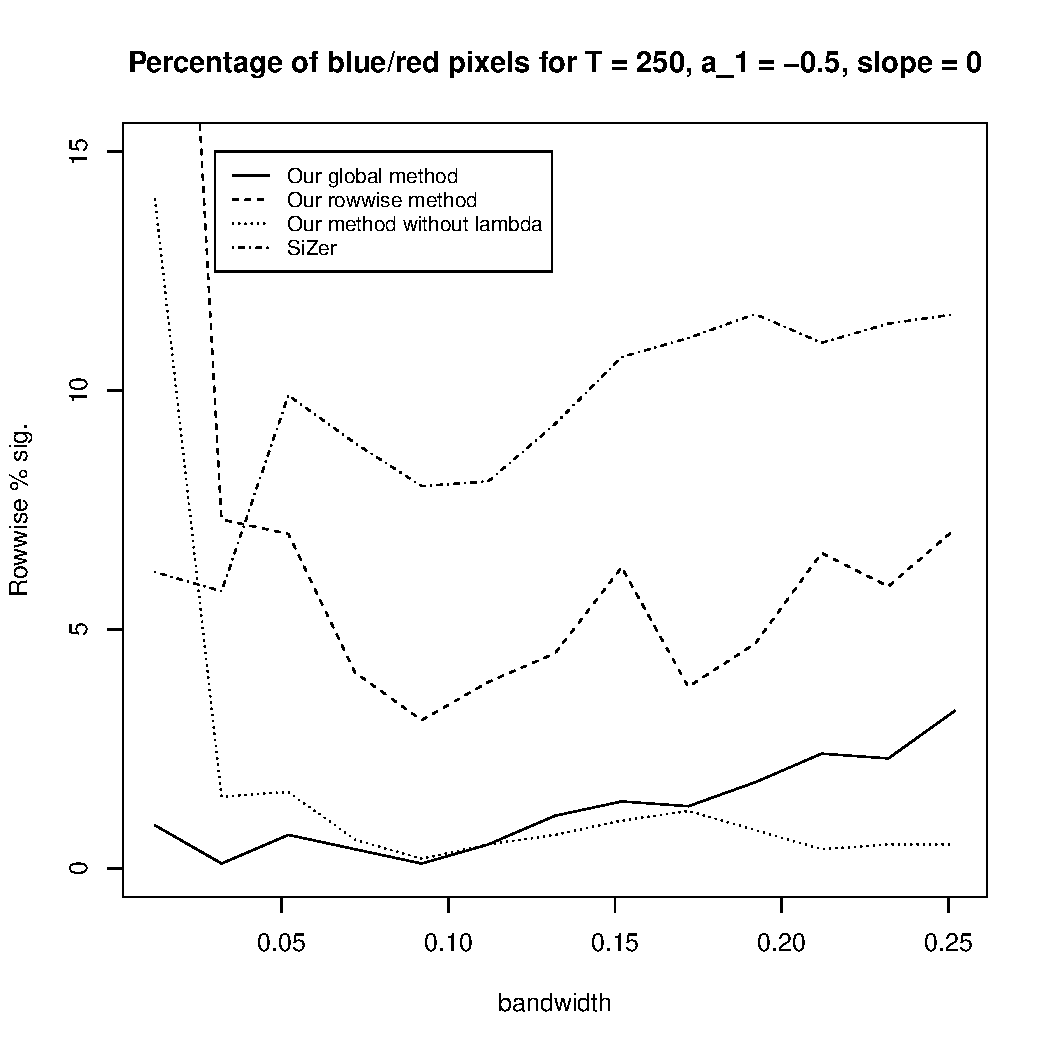
\includegraphics[width=\textwidth]{Plots/rowwise_sig_comparison_T_250_a1_-50_slope_0.pdf}
\caption{$a_1 = -0.5$, slope = $0$}
\end{subfigure}\hspace{0.25cm}
\begin{subfigure}[b]{0.475\textwidth}
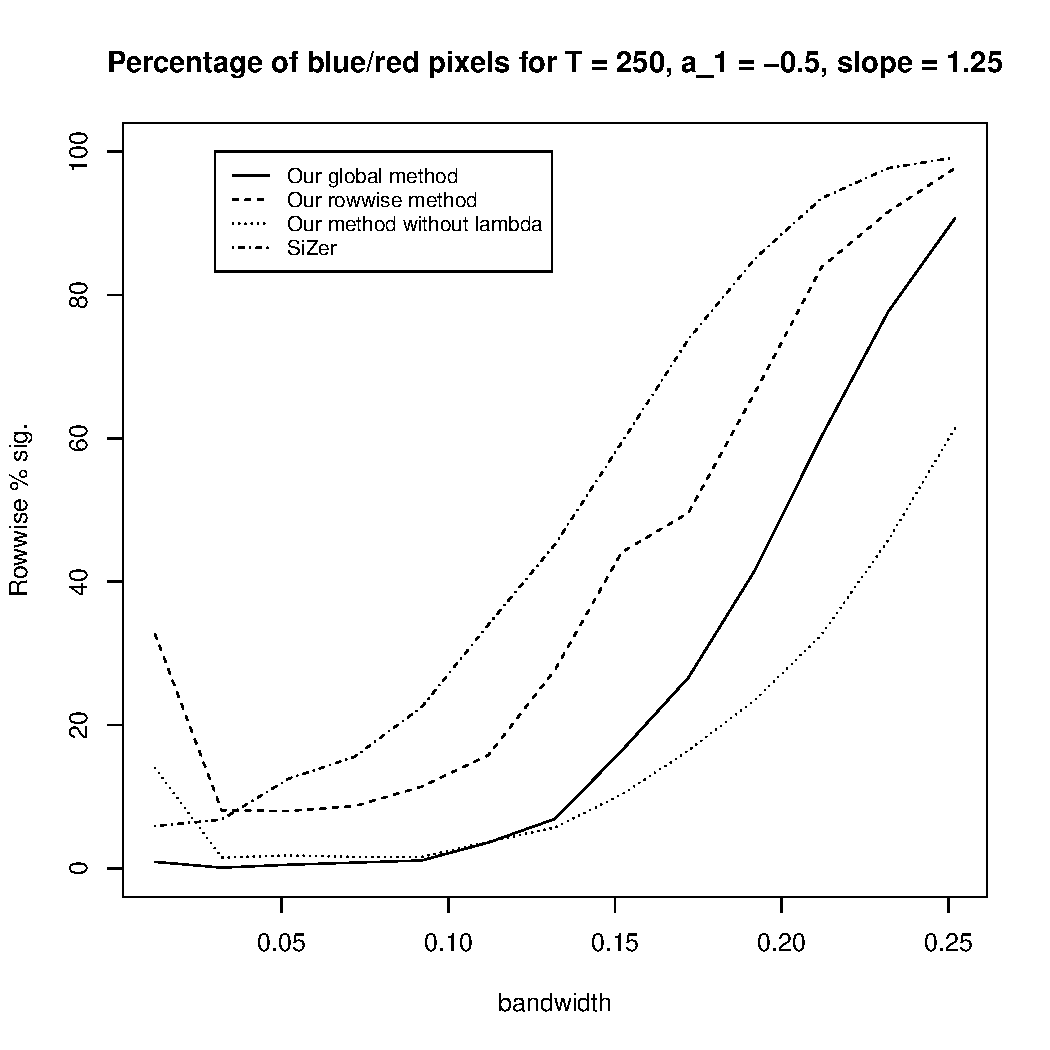
\includegraphics[width=\textwidth]{Plots/rowwise_sig_comparison_T_250_a1_-50_slope_125.pdf}
\caption{$a_1 = -0.5$, slope = $1,25$}
\end{subfigure}\\
\begin{subfigure}[b]{0.475\textwidth}
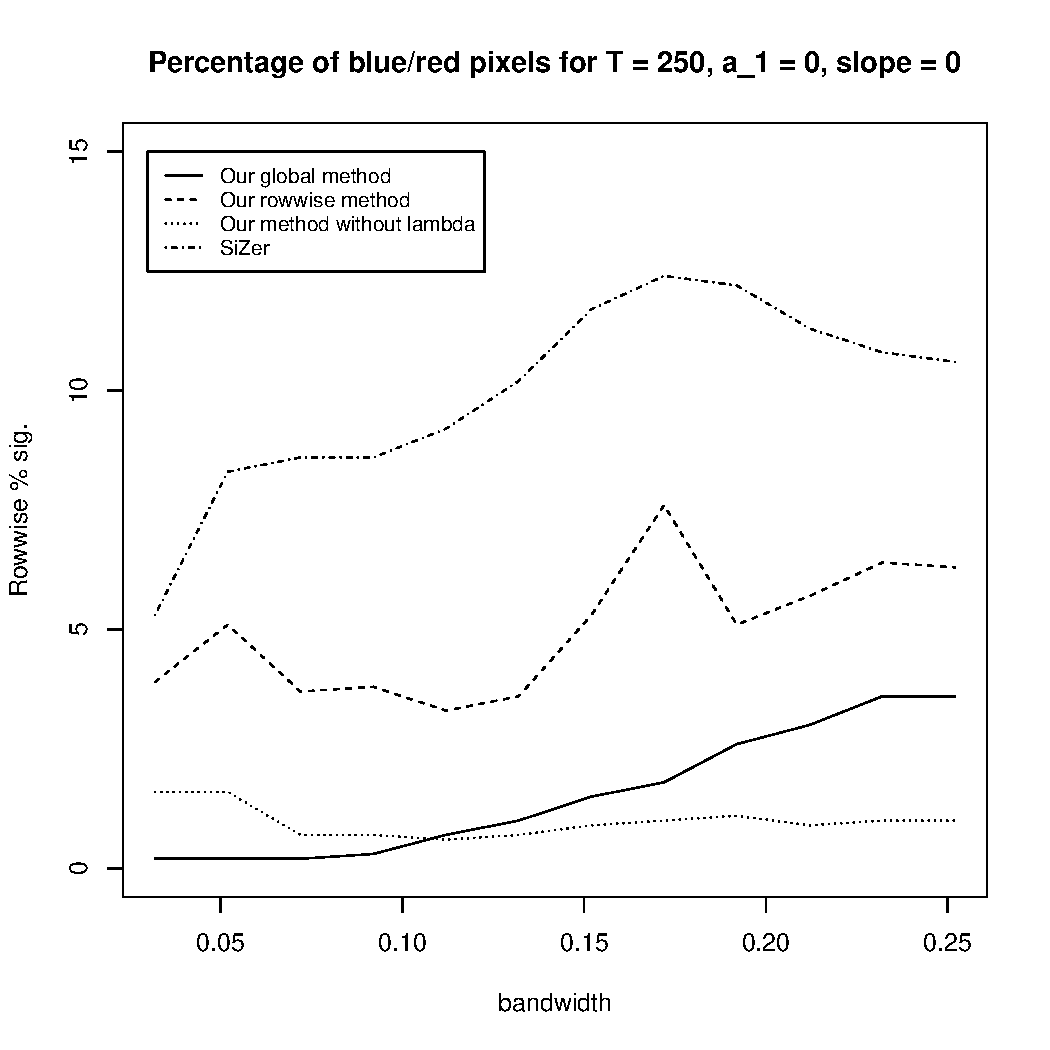
\includegraphics[width=\textwidth]{Plots/rowwise_sig_comparison_T_250_a1_0_slope_0.pdf}
\caption{$a_1 = 0$, slope = $0$}
\end{subfigure}\hspace{0.25cm}
\begin{subfigure}[b]{0.475\textwidth}
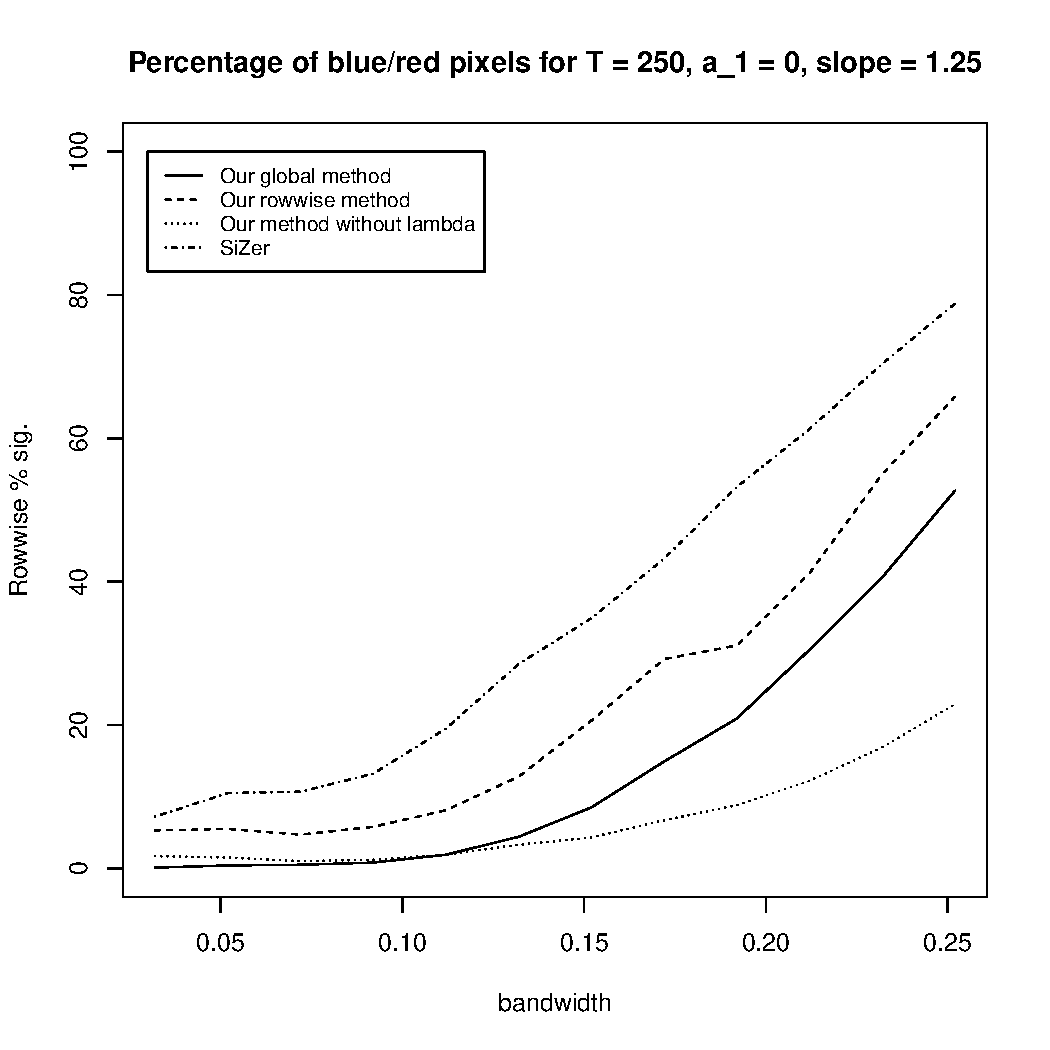
\includegraphics[width=\textwidth]{Plots/rowwise_sig_comparison_T_250_a1_0_slope_125.pdf}
\caption{$a_1 = 0$, slope = $1.25$}
\end{subfigure}\\
\begin{subfigure}[b]{0.475\textwidth}
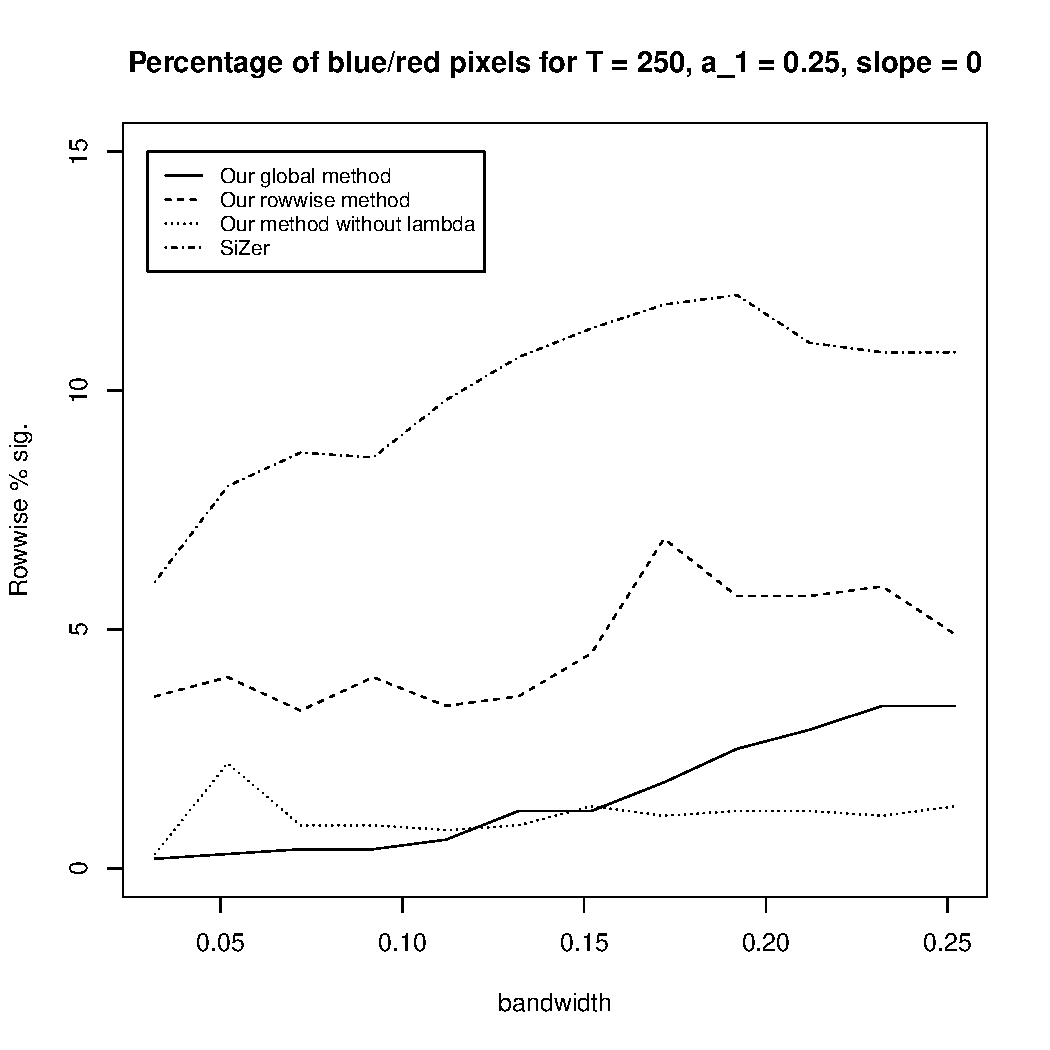
\includegraphics[width=\textwidth]{Plots/rowwise_sig_comparison_T_250_a1_25_slope_0.pdf}
\caption{$a_1 = 0.25$, slope = $0$}
\end{subfigure}\hspace{0.25cm}
\begin{subfigure}[b]{0.475\textwidth}
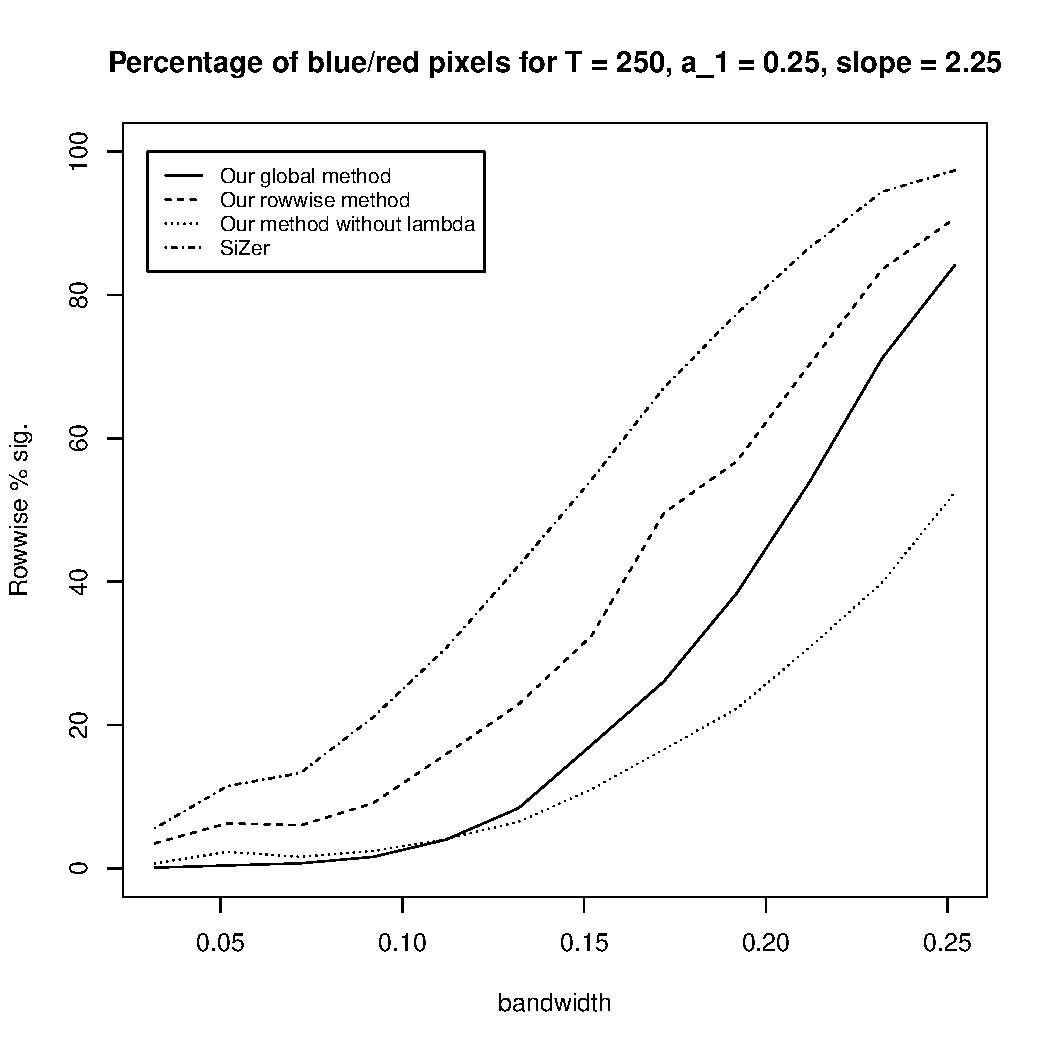
\includegraphics[width=\textwidth]{Plots/rowwise_sig_comparison_T_250_a1_25_slope_225.pdf}
\caption{$a_1 = 0.25$, slope = $2.25$}
\end{subfigure}
\caption{Parallel coordinate plots for $T = 250$ and different AR(1) parameters $a_1 = -0.5, 0, 0.25$ in the simulation scenarios with a pronounced trend and without the trend respectively.}\label{fig:PCP}
\end{figure}

\begin{figure}[t!]
\begin{subfigure}[b]{0.475\textwidth}
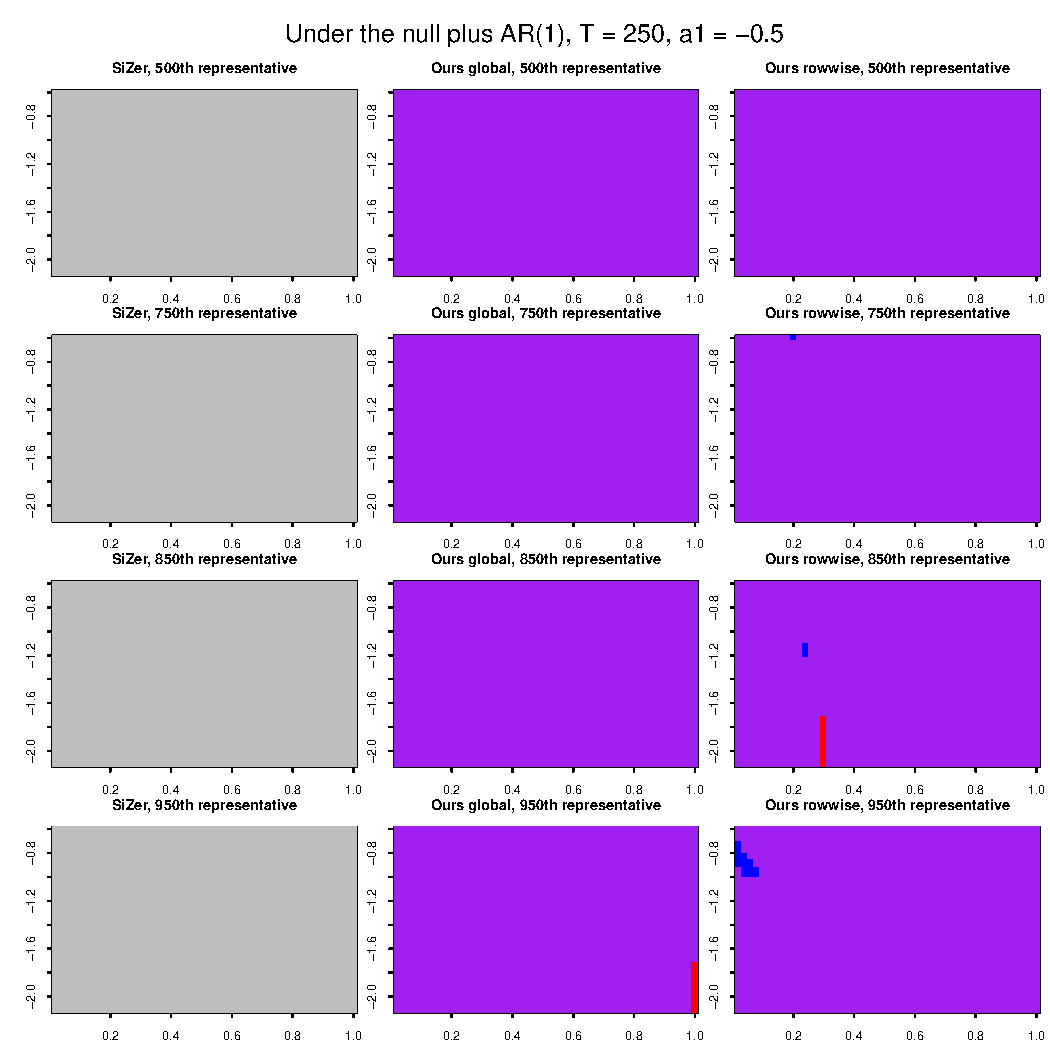
\includegraphics[width=\textwidth]{Plots/representatives_T_250_a1_-50_slope_0.pdf}
\caption{$a_1 = -0.5$}
\end{subfigure}\hspace{0.25cm}
\begin{subfigure}[b]{0.475\textwidth}
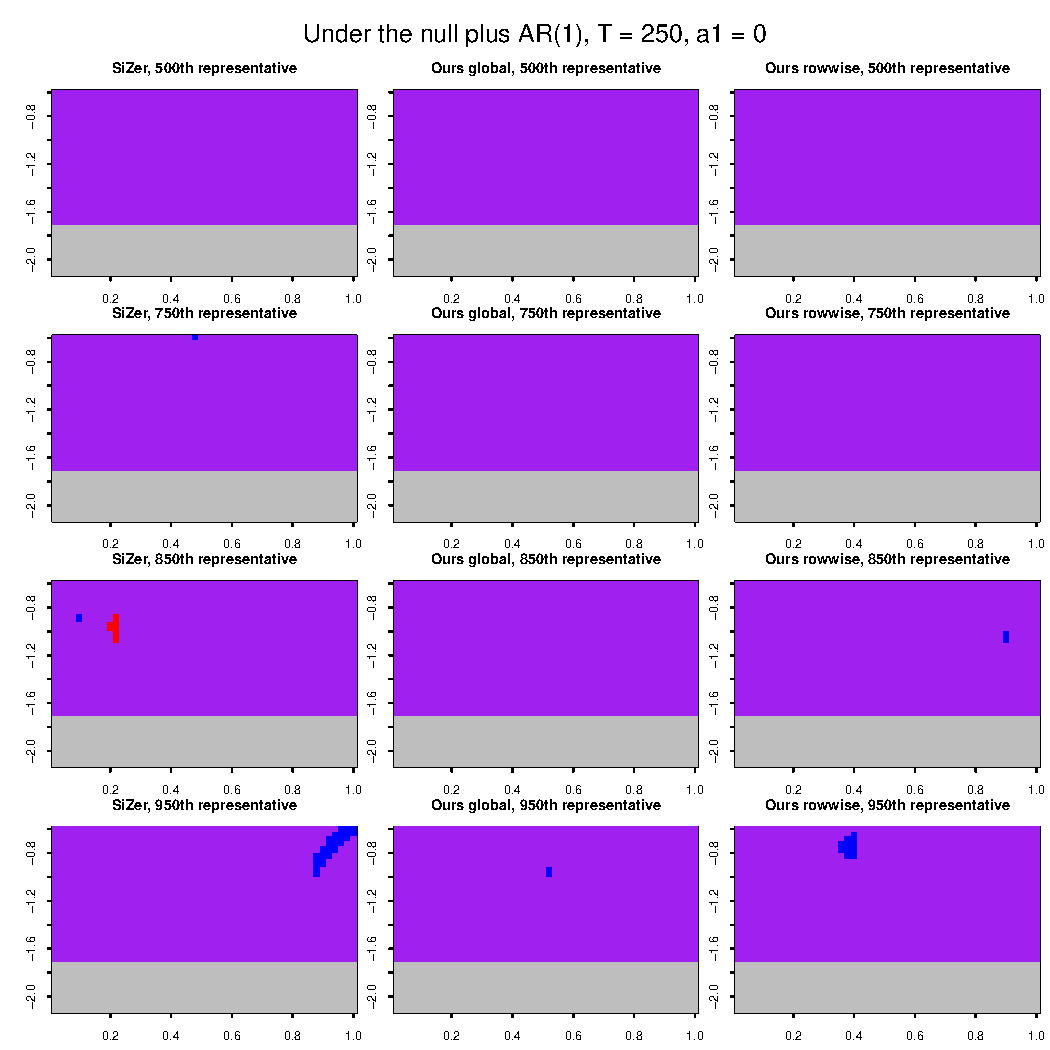
\includegraphics[width=\textwidth]{Plots/representatives_T_250_a1_0_slope_0.pdf}
\caption{$a_1 = 0$}
\end{subfigure}\\
\begin{subfigure}[b]{0.475\textwidth}
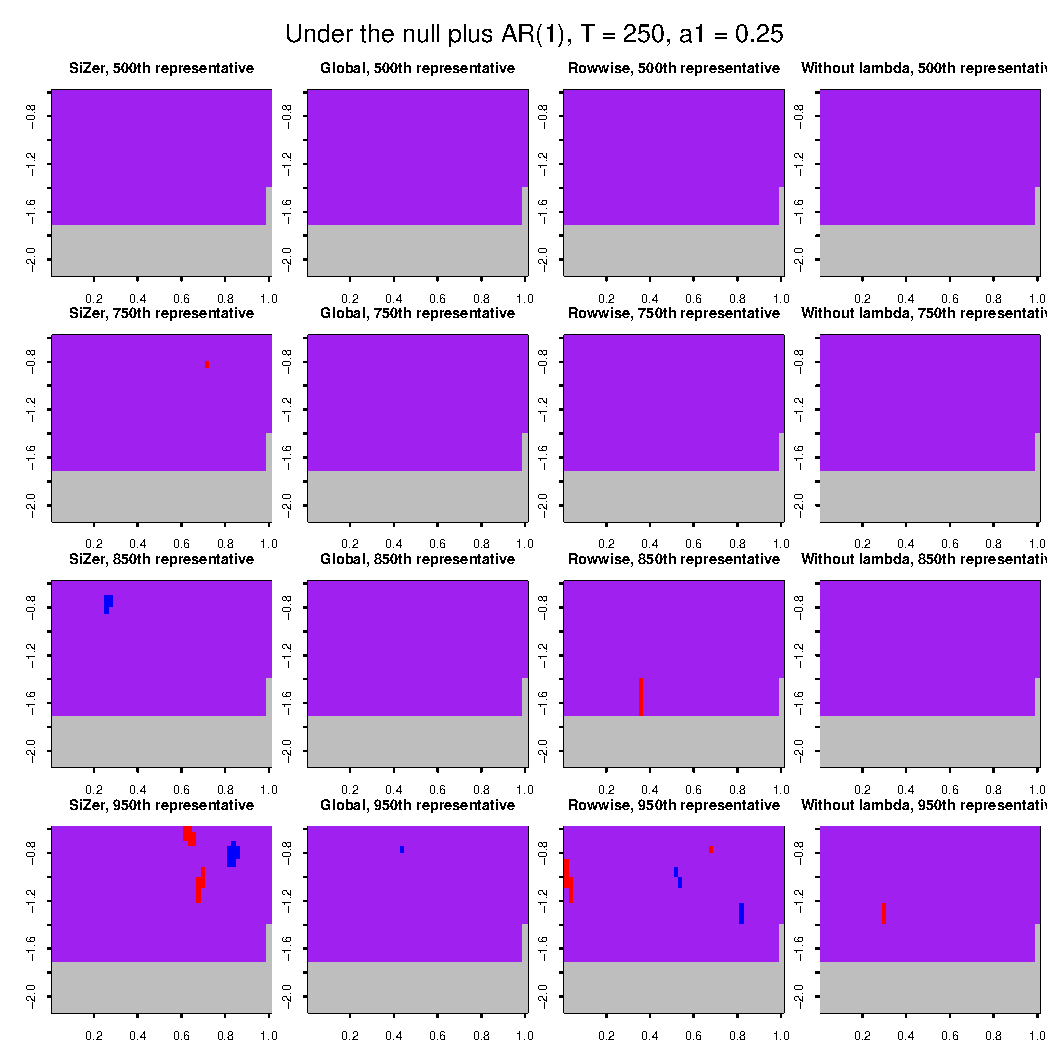
\includegraphics[width=\textwidth]{Plots/representatives_T_250_a1_25_slope_0.pdf}
\caption{$a_1 = 0.25$}
\end{subfigure}
\caption{Representative SiZer maps $T = 250$ and different AR(1) parameters $a_1 = -0.5, 0, 0.25$ in the simulation scenario under the null.}\label{fig:Representative_SiZer_maps}
\end{figure}


\bibliographystyle{ims}
{\small
\setlength{\bibsep}{0.55em}
\bibliography{bibliography}}


\end{document}
